I will focuse in this chapter on VR applications found in the literature for the visualization of bioinformatic data.

\section{Virtual Reality Chemical Space}
Virtual Reality Chemical Space is a VR application for the interactive exploartion of chemical space populated by Drugbank compounds\cite{drugbank}. It is also developed in Unity using C\# and the VRTK library. They use a particle system to render the particles of the chemical space. To render the particles, they use shaders instead of geometrical spheres as well, optimizing the number of vertices per datapoint in the scene. In order to reduce the motion sickness they have introduced a floor in the form of a grid acting as a static frame of reference. Also instead of letting the user move through the VR environment, they use a controller to move the point cloud. In Figure \ref{fig:drugbank} we can see an screenshot from the VR application. As we can notice in the screenshot, there is a subtle rendering of an outer space scene as an independent visual background. This is another technique to reduce the motion sickness that helps the user keep the notion of space. This is an interesting technique that we could have tried in BigNet VR.

They conclude in the article that the application that they have developed doesn't visualize an environment with an analogue in the real world, but instead a mathematical construct. Also some of the drawbacks that VR has compared to traditional solutions is that the VR headsets are not so comfortable as well as often-occurring eye strain and virtual reality sickness. They also conlcude that the application of VR in chemistry has more potential in the fields of education and training as for the current state of technology. The tools for chemistry need to be further evaluated wether they should be extended to VR.

\begin{figure}[h!]
    \centering%
    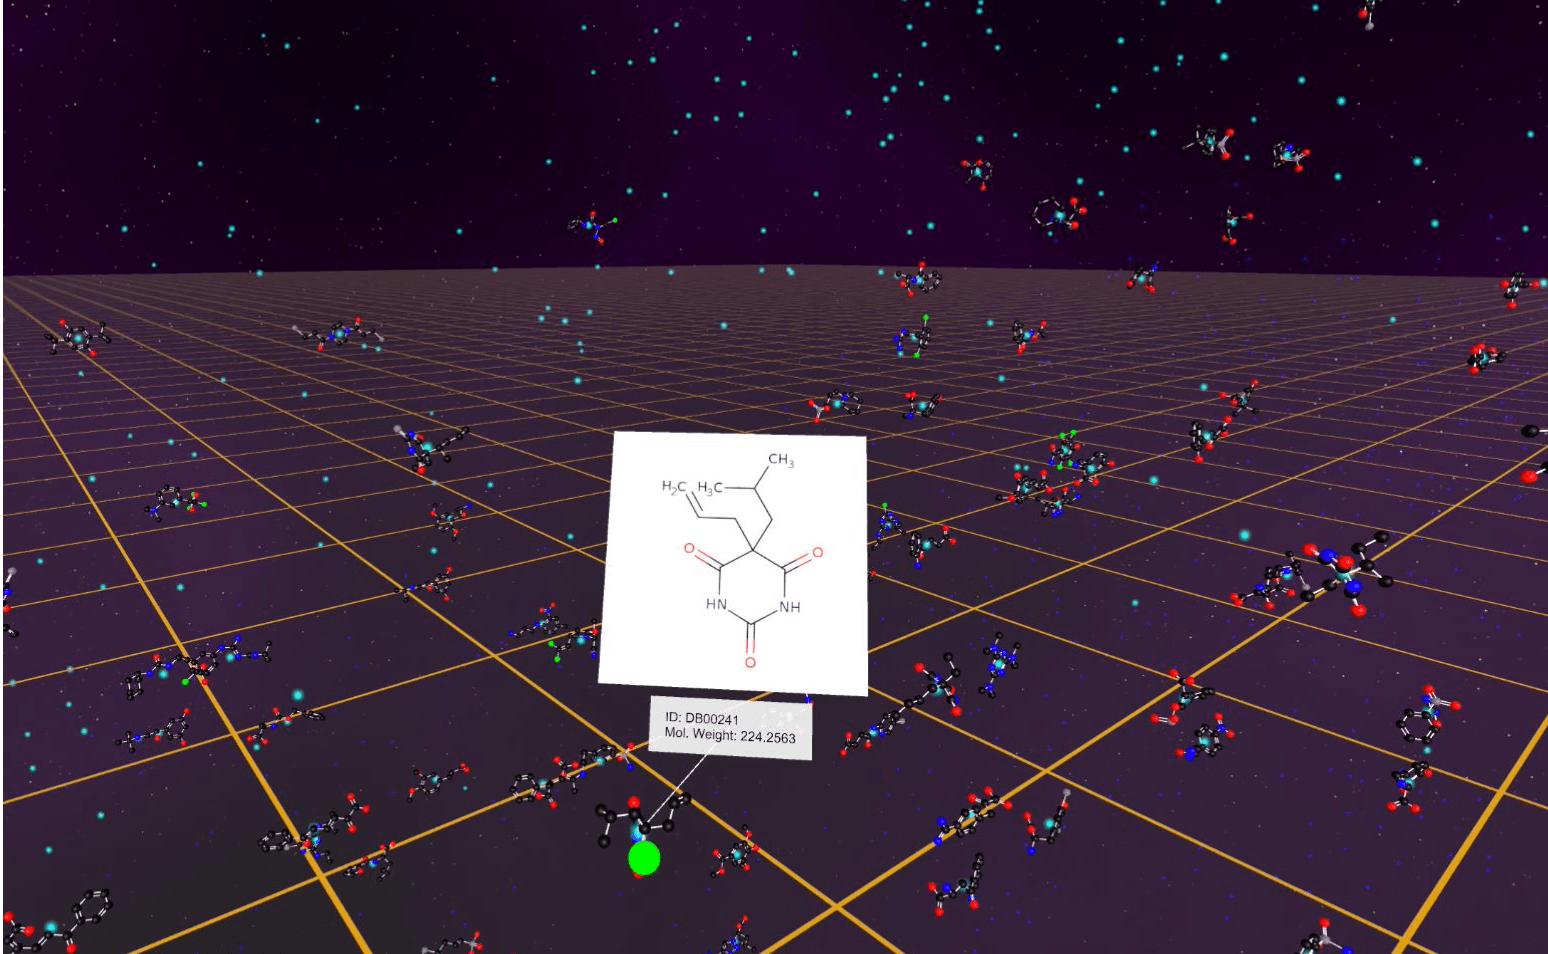
\includegraphics[width=\textwidth]{drugbank}
    \caption{Optimized virtual reality chemical space. Figure taken from \cite{drugbank}.}
    \label{fig:drugbank}
\end{figure}%

\section{BioVR}

\section{CellexaVR}

\section{BigTop}
